\documentclass[10pt,aspectratio=169]{beamer}

\usepackage[utf8]{inputenc}
\usepackage[T1]{fontenc}

\usepackage{lmodern}

\usepackage{datetime}

\usepackage{svg}
\usepackage{graphicx}
\usepackage{pdfpages}

\usepackage{multirow}

\usepackage{xcolor,colortbl}

\usepackage{soul}
\makeatletter
\newcommand\SoulColor{%
  \let\set@color\beamerorig@set@color
  \let\reset@color\beamerorig@reset@color}
\makeatother
\newcommand{\hlc}[2][yellow]{ {\sethlcolor{#1} \hl{#2}} }

\usepackage{adjustbox}

\usepackage{tikz}
\usepackage{pgfplots}
\usetikzlibrary{arrows.meta,shapes}

\date[{\tt \jobname}]{\today}
\title[TSTU]{Team Lab NLP -- Mid-term Progress Report\\Emotion Detection on Tweets}
\author[Tannert]{Touhidul Alam \& Simon Tannert}
\institute[IMS]{IMS, Universit\"at Stuttgart}

\begin{document}

\begin{frame}
  \titlepage
\end{frame}

\begin{frame}
  \frametitle{Outline}
  \tableofcontents
\end{frame}

\section{Task Description}

\begin{frame}
  \frametitle{Task Description}
  \begin{itemize}
    \item Emotion Detection is a subtask of Sentiment Analysis
    \begin{itemize}
      \item Used to find out feelings towards products, topics, etc.
      \item Companies can use it to assess the quality of their services, public figures their popularity
    \end{itemize}
    \item We were provided with a ~1.63 million tweet corpus
    \begin{itemize}
      \item Comprises tweets which use one of 8 emotions in a hashtag (e.g. \#happy)
      \item Distribution of emotion classes:\\~\\
        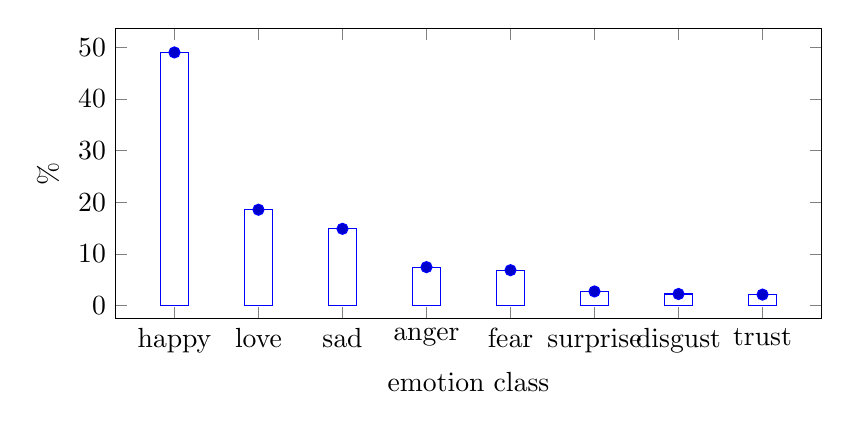
\begin{tikzpicture}
        \begin{axis}[
        height=150pt,
        width=300pt,
        xlabel=emotion class,
        ylabel=\%,
        ytick={0,10,20,30,40,50},
        xticklabels={,happy,love,sad,anger,fear,surprise,disgust,trust}]
        \addplot+[ybar] plot coordinates
          {(0,48.98) (1,18.57) (2,14.88) (3,7.47) (4,6.88) (5,2.77) (6,2.28) (7,2.16)};
        \end{axis}
        \end{tikzpicture}
    \end{itemize}
  \end{itemize}
\end{frame}

\section{Approach}

\begin{frame}
  \frametitle{Approach}
  \begin{itemize}
    \item We use the body of the tweets as only information source
    \item We extract features from the text in the body
    \item We train a Naive Bayes and a Perceptron classifier with these features
  \end{itemize}
\end{frame}

\section{Experimental Design}

\begin{frame}
  \frametitle{Experimental Design}
  \begin{itemize}
    \item We use the training set (75\%) for training and the dev set (25\%) for evaluation
    \item Only boolean features
    \begin{itemize}
      \item All tokens are normalized to lowercase
      \item ``@\$\{username\}'' is normalized to ``@USERNAME''
    \end{itemize}
    \item Two sources of features:
    \begin{itemize}
      \item Bag of words
      \item Concatenation of two consecutive words
    \end{itemize} 
  \end{itemize}~\\
  Naive Bayes:
  \begin{itemize}
    \item Uses Laplace smooting with $\alpha=0.06$ for unseen words
  \end{itemize}~\\
  Perceptron:
  \begin{itemize}
    \item The training data is shuffled before every epoch
  \end{itemize}
\end{frame}

\section{Results}

\begin{frame}
  \frametitle{Results}
  % \framesubtitle{Naive Bayes classifier}
  \textbf{Naive Bayes classifier}
  \begin{tabular}{r|llllllll}
              & anger & disgust & fear  & happy & love  & sad   & surprise & trust\\\hline
    Precision & 77.59 & 100.00  & 64.57 & 65.18 & 51.78 & 57.33 & 64.06    & 37.50\\
    Recall    & 30.95 & 14.03   & 41.53 & 79.79 & 44.66 & 70.38 & 15.77    & 0.40\\
    F1-Score  & 44.25 & 24.61   & 50.55 & 71.75 & 47.96 & 63.19 & 25.31    & 0.78\\
  \end{tabular}\\~\\
  Macro Average F1-Score: 41.05\\
  Accuracy: 62.02\\~\\
 
  \textbf{Perceptron classifier} (after 13 epochs)
  \begin{tabular}{r|llllllll}
              & anger & disgust & fear  & happy & love  & sad   & surprise & trust\\\hline
    Precision & 75.80 & 66.18   & 67.84 & 72.24 & 66.48 & 71.14 & 62.93    & 43.89\\
    Recall    & 58.81 & 34.20   & 59.30 & 85.09 & 54.49 & 71.89 & 32.97    & 18.49\\
    F1-Score  & 66.23 & 45.10   & 63.29 & 78.14 & 59.89 & 71.51 & 43.27    & 26.02\\
  \end{tabular}\\~\\

  Macro Average F1-Score: 56.68\\
  Accuracy: 71.09
 
\end{frame}

\section{Next Steps}

\begin{frame}
  \frametitle{Next Steps}
  \begin{itemize}
    \item 31\% of tweets in the training set and 25\% in the dev
      set come with an image
    \item We want to use the image as an additional source of information
    \item Simple approach:
    \begin{itemize}
      \item Split the image into subframes evenly and calculate the median color value
      \item Extract brightness, hue and saturation from each pixel
        \begin{tikzpicture}
          \node(a){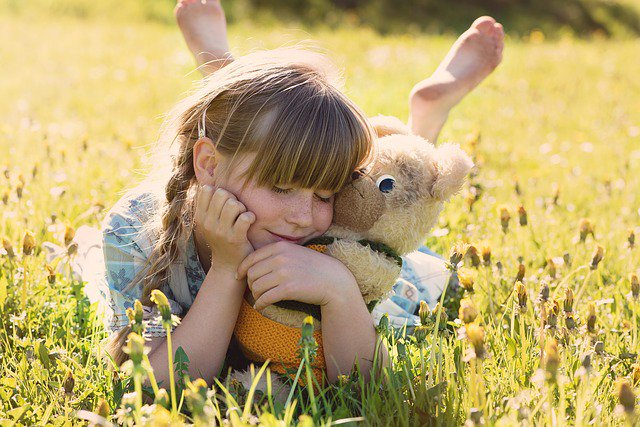
\includegraphics[scale=.12]{../res/804855952797270016.jpg}};
          \node(b)[right of=a,xshift=60pt,yshift=-10pt]{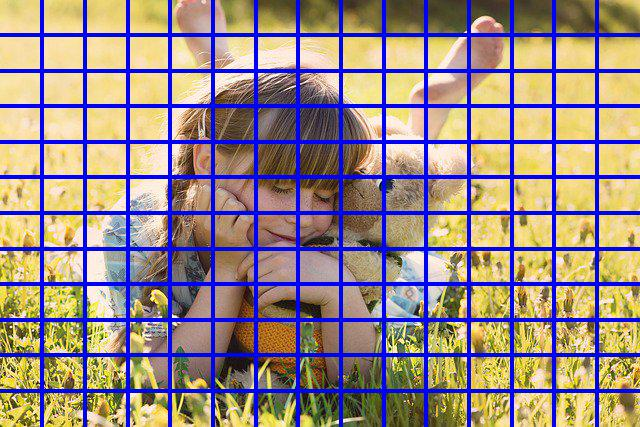
\includegraphics[scale=.12]{../res/804855952797270016_grid.jpg}};
          \node(c)[right of=b,xshift=60pt,yshift=-10pt]{
\includegraphics[scale=.12]{../res/804855952797270016_med.jpg}};
          \node(d)[below of=c,xshift=-85pt,yshift=-35pt]{
\includegraphics[scale=.12]{../res/804855952797270016_lum.jpg}};
          \node(e)[below of=c,xshift=0pt,yshift=-35pt]{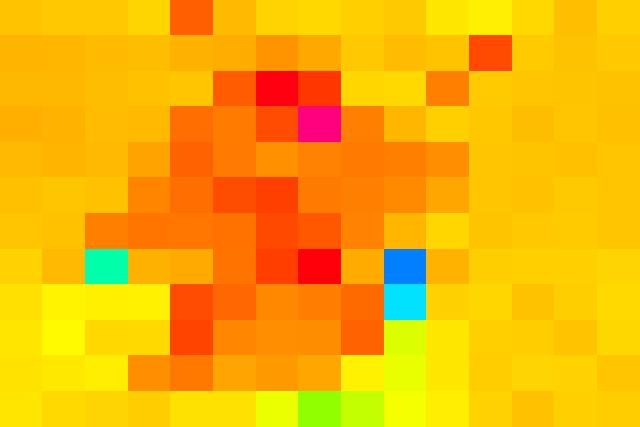
\includegraphics[scale=.12]{../res/804855952797270016_hue.jpg}};
          \node(f)[below of=c,xshift=85pt,yshift=-35pt]{
\includegraphics[scale=.12]{../res/804855952797270016_sat.jpg}};

          \node(hd)[below of=d,yshift=-5pt] {B};
          \node(he)[below of=e,yshift=-5pt] {H};
          \node(hf)[below of=f,yshift=-5pt] {S};

          \draw[->](a) -- (b);
          \draw[->](b) -- (c);
          \draw(c) -- (d);
          \draw(c) -- (e);
          \draw(c) -- (f);
        \end{tikzpicture}\vspace*{-0pt}
    \end{itemize}
  \end{itemize}
\end{frame}

\begin{frame}
  \frametitle{Next Steps}
  \begin{itemize}
  \item[]
    \begin{itemize}
      \item Reduce the dimensionality of the raw brightness, hue and saturation values
  %  \end{itemize}
  % \end{itemize}
    %% \vspace*{-40pt}\hspace*{20pt}\begin{tikzpicture}
    %%       \node(a){\includegraphics[scale=.12]{res/687689314550046721.jpg}};
    %%       \node(b)[below of=a,xshift=-70pt,yshift=-50pt]{\includegraphics[scale=.12]{res/687689314550046721_lum.jpg}};
    %%       \node(c)[below of=a,xshift=0pt,yshift=-50pt]{\includegraphics[scale=.12]{res/687689314550046721_hue.jpg}};
    %%       \node(d)[below of=a,xshift=70pt,yshift=-50pt]{\includegraphics[scale=.12]{res/687689314550046721_sat.jpg}};

    %%       \draw(a) -> (b);
    %%       \draw(a) -> (c);
    %%       \draw(a) -> (d);
    %%     \end{tikzpicture}\vspace*{-20pt}

  \begin{minipage}{.4\textwidth}
  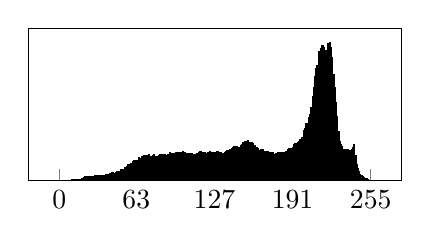
\begin{tikzpicture}
    \begin{axis}[
        ymin=0,
        height=100pt,
        width=180pt,
        xtick pos=left,
        xtick={0,63,127,191,255},
        ytick=\empty,
      ]
      \addplot[ybar interval,mark=no,fill=black] plot coordinates { (0,0.000000) (1,0.001098) (2,0.002196) (3,0.001464) (4,0.002927) (5,0.002561) (6,0.000732) (7,0.002927) (8,0.003293) (9,0.003293) (10,0.008782) (11,0.004391) (12,0.007684) (13,0.006221) (14,0.008050) (15,0.015735) (16,0.015369) (17,0.016101) (18,0.024151) (19,0.024151) (20,0.040984) (21,0.044643) (22,0.048668) (23,0.051961) (24,0.054157) (25,0.055987) (26,0.056352) (27,0.053791) (28,0.042447) (29,0.057084) (30,0.060744) (31,0.054523) (32,0.058182) (33,0.063305) (34,0.065867) (35,0.062573) (36,0.062939) (37,0.068794) (38,0.074283) (39,0.071721) (40,0.067330) (41,0.094775) (42,0.089286) (43,0.097702) (44,0.093677) (45,0.092579) (46,0.102093) (47,0.111973) (48,0.110509) (49,0.118194) (50,0.136856) (51,0.135758) (52,0.145272) (53,0.162105) (54,0.171253) (55,0.173814) (56,0.211505) (57,0.203454) (58,0.213700) (59,0.216262) (60,0.238583) (61,0.259441) (62,0.260173) (63,0.259441) (64,0.261636) (65,0.294570) (66,0.286153) (67,0.307011) (68,0.290544) (69,0.323112) (70,0.317623) (71,0.321648) (72,0.307743) (73,0.332260) (74,0.295667) (75,0.308475) (76,0.315061) (77,0.337017) (78,0.314696) (79,0.305181) (80,0.313232) (81,0.318721) (82,0.334821) (83,0.338481) (84,0.333358) (85,0.317257) (86,0.337017) (87,0.312134) (88,0.315061) (89,0.339944) (90,0.354947) (91,0.345067) (92,0.352386) (93,0.346531) (94,0.327869) (95,0.362998) (96,0.357875) (97,0.357875) (98,0.357509) (99,0.344335) (100,0.357875) (101,0.367389) (102,0.356411) (103,0.345433) (104,0.345067) (105,0.348361) (106,0.352752) (107,0.331894) (108,0.341042) (109,0.330064) (110,0.339213) (111,0.339944) (112,0.345067) (113,0.351654) (114,0.361534) (115,0.369584) (116,0.355313) (117,0.358972) (118,0.366291) (119,0.362632) (120,0.346531) (121,0.360436) (122,0.361900) (123,0.372512) (124,0.362632) (125,0.349093) (126,0.364095) (127,0.354947) (128,0.342140) (129,0.369950) (130,0.355313) (131,0.362998) (132,0.360070) (133,0.341042) (134,0.351654) (135,0.365559) (136,0.373975) (137,0.382392) (138,0.381660) (139,0.401054) (140,0.391174) (141,0.413861) (142,0.419350) (143,0.436549) (144,0.438378) (145,0.436915) (146,0.428864) (147,0.423009) (148,0.456674) (149,0.462163) (150,0.494731) (151,0.473507) (152,0.501683) (153,0.495828) (154,0.510100) (155,0.478630) (156,0.486680) (157,0.493633) (158,0.476434) (159,0.445331) (160,0.451552) (161,0.426303) (162,0.415691) (163,0.379830) (164,0.376903) (165,0.395931) (166,0.395199) (167,0.363364) (168,0.375073) (169,0.371780) (170,0.371780) (171,0.352386) (172,0.359338) (173,0.357143) (174,0.355313) (175,0.321648) (176,0.335553) (177,0.352752) (178,0.326039) (179,0.361168) (180,0.351288) (181,0.365559) (182,0.331162) (183,0.356045) (184,0.338847) (185,0.367755) (186,0.371780) (187,0.393369) (188,0.408738) (189,0.414593) (190,0.414227) (191,0.419350) (192,0.459602) (193,0.475703) (194,0.450454) (195,0.484851) (196,0.499488) (197,0.522907) (198,0.554742) (199,0.545228) (200,0.638173) (201,0.672204) (202,0.728557) (203,0.733314) (204,0.810890) (205,0.848214) (206,0.948112) (207,1.084602) (208,1.195111) (209,1.338188) (210,1.441013) (211,1.485290) (212,1.671546) (213,1.664593) (214,1.701917) (215,1.737412) (216,1.718384) (217,1.678132) (218,1.678864) (219,1.671180) (220,1.762661) (221,1.787910) (222,1.716920) (223,1.589944) (224,1.370755) (225,1.199868) (226,1.006294) (227,0.820038) (228,0.631587) (229,0.508636) (230,0.463993) (231,0.432523) (232,0.397029) (233,0.397029) (234,0.389344) (235,0.396297) (236,0.395199) (237,0.382758) (238,0.380196) (239,0.393369) (240,0.428864) (241,0.468018) (242,0.320916) (243,0.207480) (244,0.147468) (245,0.110143) (246,0.077210) (247,0.057084) (248,0.050864) (249,0.037324) (250,0.024151) (251,0.020858) (252,0.007319) (253,0.002196) (254,0.000000) (255,0.000000) };
    \end{axis}
  \end{tikzpicture}
  \end{minipage}\begin{minipage}{.5\textwidth}
  \vspace*{22pt}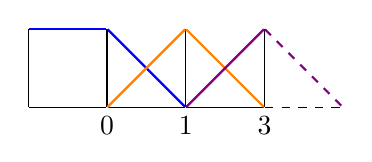
\begin{tikzpicture}[every node/.style={inner sep=0pt,minimum size=0pt}]
    \node(a)[draw=none] {};
    \node(b)[draw=none,right of=a] {};
    \node(c)[draw=none,right of=b] {};
    \node(d)[draw=none,right of=c] {};
    \node(e)[draw=none,right of=d] {};

    \node(bl)[draw=none,below of=b,yshift=22pt] {0};
    \node(cl)[draw=none,below of=c,yshift=22pt] {1};
    \node(dl)[draw=none,below of=d,yshift=22pt] {3};

    \node(at)[draw=none,above of=a] {};
    \node(bt)[draw=none,above of=b] {};
    \node(ct)[draw=none,above of=c] {};
    \node(dt)[draw=none,above of=d] {};

    \path[draw=black](a) -- (b);
    \path[draw=black](b) -- (c);
    \path[draw=black](c) -- (d);
    \path[draw=black,dashed](d) -- (e);

    \path[draw=black](a) -- (at);
    \path[draw=black](b) -- (bt);
    \path[draw=black](c) -- (ct);
    \path[draw=black](d) -- (dt);

    \path[draw=blue,thick](at) -- (bt);
    \path[draw=blue,thick](bt) -- (c);
    \path[draw=orange,thick](b) -- (ct);
    \path[draw=orange,thick](ct) -- (d);
    \path[draw=violet,thick](c) -- (dt);
    \path[draw=violet,thick,dashed](dt) -- (e);

  \end{tikzpicture}
  \end{minipage}

  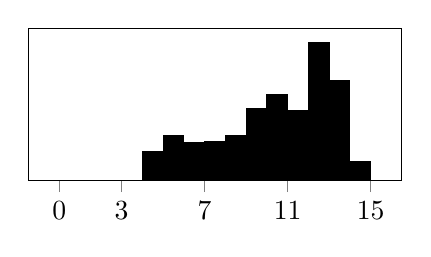
\begin{tikzpicture}
    \begin{axis}[
        ymin=0,
        height=100pt,
        width=180pt,
        xtick pos=left,
        xtick={0,3,7,11,15},
        ytick=\empty,
        bar width=1cm,
        ybar=-1.5cm,
      ]
      \addplot[ybar interval,mark=no,fill=black] plot coordinates { (0,0.0) (1,0.0) (2,0.0) (3,0.0) (4,4.228571428571429) (5,6.552380952380952) (6,5.561904761904762) (7,5.752380952380952) (8,6.59047619047619) (9,10.59047619047619) (10,12.647619047619047) (11,10.285714285714286) (12,20.266666666666666) (13,14.59047619047619) (14,2.8190476190476192) (15,0.11428571428571428) };
    \end{axis}
  \end{tikzpicture}

  \item Train our perceptron with the extracted features
  \end{itemize}
  %\begin{itemize}
    \item Better approach:
    \begin{itemize}
      \item Train a convolutional neural network (CNN) to predict emotions
        based on the images
      \item Combine this with a neural network that learns to predict emotions from the text
    \end{itemize}
    \item Touhidul will finish the Perceptron based image classificator, Simon will start implementing the CNN
  \end{itemize}
\end{frame}

\end{document}
